\section{Design}
\label{sec:design}

This chapter presents the implemented framework \textit{Banshie} (Benchmark Framework for Information Extraction). The requirements, architecture, design and concrete implementation details are explained and discussed on the following pages.

\subsection{Analysis and requirements}
The main goal was to provide a platform to benchmark domain-specific information extraction modules. Since the framework is planned to be used in a bigger platform and by other developers, it had to be designed for extension, modularity and embeddability. It should be based on the OSGi infrastructure and build with state-of-the-art patterns, like \gls{DI}, \gls{IoC} and Composition over Inheritance in mind.

Since Banshie had to be developed in an Open Source fashion to support broader use cases, its whole code base as well as the  documentation is available via

\url{https://github.com/whiskeysierra/banshie}

\subsection{Architecture}
Banshie is completely written in Java and distributed as OSGi bundles. The architecture of the framework was not the result of a \gls{BDUF} but is rather based on a very rough design idea which allows to incrementally build in the design details as the project progresses. \citeauthor{Knoernschild:2012} provides a catalog of architectural patterns for building highly modular systems in his book: \citetitle{Knoernschild:2012} \cite{Knoernschild:2012}

Almost all of Banshie's modules are the result of applying these patterns during the development. The following figure shows all relevant modules as well as their dependencies.

\newpage
\begin{figure}[H]
\centering
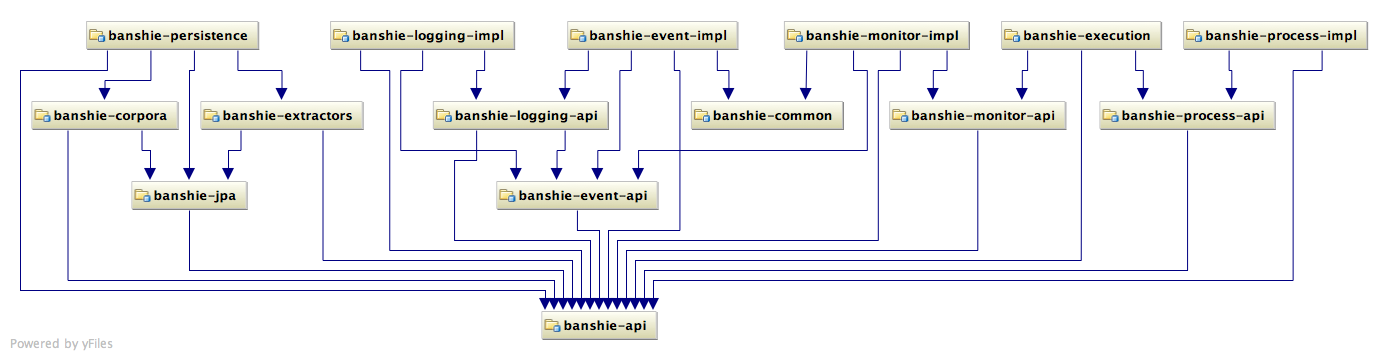
\includegraphics[angle=90, width=0.38\textwidth]{module-dependencies.png}
\caption{Module dependencies}
\label{fig:module-dependencies}
\end{figure}

\newpage
\subsection{Technologies and patterns}

\subsubsection{Dependency Injection}
\gls{DI} is an expression introduced by Martin Fowler in its article \textit{Inversion of Control Containers and the Dependency Injection Pattern} \cite{Fowler:2004}. Dependency Injection specifies the means for obtaining objects in such a way as to maximize reusability, testability and maintainability compared to traditional approaches such as constructors, factories, and service locators \cite{JSR330}. \gls{DI} does this by allowing a class to specify its dependencies and rely on their provision at runtime rather than retrieving them explicitly. This leaves the programmer's code clean, flexible, and relatively free of dependency-related infrastructure \cite{JSR330}.

\paragraph{Guice}
Guice is a lightweight dependency injection framework for Java \cite{Guice}. It's Open Source and available on \url{https://code.google.com/p/google-guice/}.

The typical code to implement Guice is shown in the following two listings. The first shows a simple \textit{Module}. Modules in Guice are usually used to bind interfaces to concrete classes.

\begin{listing}[H]
\begin{minted}{java}
public final class ProcessModule extends AbstractModule {

    @Override 
    protected void configure() {
        bind(ProcessService.class).to(DefaultProcessService.class);
    }

}
\end{minted}
\caption{Guice module}
\end{listing}

In your classes you usually define a single constructor, annotated with \texttt{@Inject}, and all required dependencies as parameters. The construction of instances and the dependency resolution is done by Guice, no additional boilerplate code is necessary.

\begin{listing}[H]
\begin{minted}{java}
final class DefaultEngine implements Engine {

    private final ProcessService service;

    @Inject
    DefaultEngine(ProcessService service) {
        this.service = service;
    }

}
\end{minted}
\caption{Constructor injection}
\end{listing}

\paragraph{Guice Extensions}
Guice has an extensible plug-in mechanism which allows third parties to provide additional functionality. Banshie uses two official Guice extension extensively: Assisted Inject\footnote{\url{https://code.google.com/p/google-guice/wiki/AssistedInject}} and Multibindings\footnote{\url{https://code.google.com/p/google-guice/wiki/Multibinding}}. Assisted Inject allows the combination of Guice-provided dependencies and user-provided parameters on a single injection point. Multibindings supports the binding and injection of Sets and Maps.

\paragraph{Peaberry}
Guice has no native OSGi support, apart from maybe the OSGi-compatible bundle manifest. To overcome this shortcoming, Peaberry\footnote{\url{https://code.google.com/p/peaberry/}}, a third-party open-source Guice extension, offers OSGi-Guice bridge capabilities. It offers \gls{DI} of OSGi dynamic services via Guice's common injection mechanisms and provides a rich and typesafe API to deal with the OSGi service registry and lifecycle events. Listing \ref{lst:peaberry-lifecycle} shows the usage of Peaberry's lifecycle annotations.

\begin{listing}[H]
\begin{minted}{java}
import org.ops4j.peaberry.activation.Start;

public class DefaultCorpusRepository implements CorpusRepository {

    private File basePath = new File("corpora");

    @Start
    public void onStart() {
        basePath.mkdirs();
    }

}
\end{minted}
\caption{Peaberry lifecycle annotation}
\label{lst:peaberry-lifecycle}
\end{listing}

Peaberry even supports the automatic \gls{DI} context creation upon bundle start by using an OSGi extender bundle. Bundles just need to provide the following bundle header to trigger an execution:

\begin{listing}[H]
\texttt{Bundle-Module: org.whiskeysierra.banshie.execution.ExecutionModule}
\caption{Peaberry bundle header}
\end{listing}

Peaberry creates one \texttt{Injector} per bundle, any interaction between bundles is based on standard OSGi services, which allows to combine Peaberry-aware bundles and normal ones.

\subsubsection{Persistence}
Banshie's persistence layer is based on the \gls{JPA} 2.0 Standard. \gls{JPA} allows to build modules without hardcoding for a specific persistence provider or database vendor. Thus allowing to swap implementations later in the development lifecycle without the need to rewrite large portions of the code base. Banshie uses Apache OpenJPA as a \gls{JPA} provider and Apache Derby as the underlying database. Derby is a \gls{RDBMS} written in Java and is distributable as a single Jar file which can be embedded in other applications rather easily.

Using \gls{JPA} in an \gls{OSGi} environment is not a straight forward task. \gls{OSGi} requires bundles to run in different and independent class loaders, while \gls{JPA} heavily relies on classpath scanning and reflection. Both techniques don't work quite well together. Because \gls{JPA}-based persistence is a common requirement, the \citetitle{OSGI:Enterprise} addressed this issue and specifies a standard way to define \textit{Persistence} and \textit{Client bundles} \cite{OSGI:Enterprise}. A persistence bundle is a bundle with the following bundle header:

\begin{listing}[H]
\texttt{Meta-Persistence: META-INF/persistence.xml}
\caption{Persistence bundle header}
\end{listing}

A client bundle is just a bundle that makes use of the \texttt{EntityManagerFactory} provided by the corresponding persistence unit. Most \gls{OSGi} containers delegate this part of the \gls{OSGi} specification to third-party libraries and bundles. Apache Aries aims to provide portable implementations in the form of standard \gls{OSGi} bundles for those parts of the \gls{OSGi} specification. Banshie uses the JPA module of Apache Aries consisting of the \textit{Aries JPA API bundle} and the \textit{Aries JPA container bundle}. To minimize common boilerplate code and manual transaction handling, all \gls{JPA} client bundles use the Guice extension \textit{Guice Persist}. Guice Persist offers AOP-interception for annotated methods as shown in the following listing:

\begin{listing}[H]
\begin{minted}{java}
class DefaultCorpusRepository implements CorpusRepository {

    private EntityManager manager() {
        return provider.get();
    }

    @Transactional
    @Override
    public Corpus get(UUID uuid) {
        return manager().find(CorpusEntity.class, uuid);
    }

}
\end{minted}
\caption{Guice Persist annotation}
\end{listing}

\subsubsection{Build tools}
\paragraph{BND Tool and the Maven Bundle Plugin}
With \gls{OSGi} you are forced to provide additional metadata in the JAR's manifest to verify the consistency of your classpath. This metadata must be closely aligned with the class files in the bundle. Maintaining this metdata is an error prone chore because many aspects are redundant. The core task of the BND Tool is to analyze the class files and find every dependency. These dependencies are then merged with instructions supplied by the user \cite{BND}. Since Banshie uses Apache Maven for building its independent modules, the natural choice was to use a Maven Plugin for this, which is provided by the Apache Felix Maven Bundle Plugin \footnote{\url{http://felix.apache.org/site/apache-felix-maven-bundle-plugin-bnd.html}}. The following listing shows the bare minimum of configuration code to use the Maven Bundle Plugin in a POM file.

\begin{listing}[H]
\begin{minted}{xml}
<packaging>bundle</packaging>
...
<build>
    <plugins>
        <plugin>
            <groupId>org.apache.felix</groupId>
            <artifactId>maven-bundle-plugin</artifactId>
        </plugin>
    </plugins>
</build>
\end{minted}
\caption{Maven Bundle Plugin usage}
\end{listing}

\newpage
\subsection{API}
The framework's \gls{API} can be divided into three main components, which are described in detail on the following pages.

\paragraph{Domain model and persistence}
Banshie's domain model has been designed with simplicity and extensibility in mind. The two only entity classes, \texttt{Corpus} and \texttt{Extractor}, are merely containers for file locations and very little meta data, but since the persistence layer is based on \gls{JPA}, which is based on \textit{Plain Old Java Objects}, adding properties is a rather easy task.

An extractor holds the name, version and the path to the executable jar file, while a corpus identifies the reference output as well as a related input document.

For each of the model classes a persistence service interface is provided. Since the framework in it current stage does not require very sophisticated features, the interface of these services is intentionally kept to a minimum.

\begin{figure}[H]
\centering
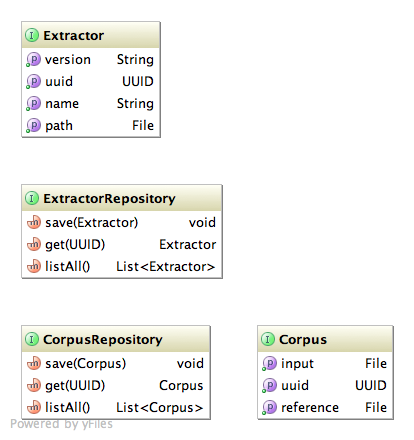
\includegraphics[width=0.8\textwidth, trim=20px 20px 0 0, clip=true]{api-model.png}
\caption{Banshie model and persistence API}
\end{figure}

\newpage
\paragraph{Execution}
Apart from the domain model and persistence layer, the framework offers two significant features to its clients: execution and evaluation. The execution package contains one major interface for executing extractors: the \texttt{Engine}. The Engine provides a single methods which takes an Extractor-Corpus-pair and performs an execution. The result of the extractor run is then passed back to the caller in the form of an \texttt{ExtractorResult} containing references to the extractor's xml output file and the event log file. For more details about the structure of the event log file please consult chapter \ref{sec:implementation}.

\begin{figure}[H]
\centering
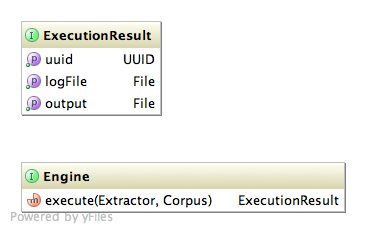
\includegraphics[width=0.7\textwidth, trim=20px 20px 0 0, clip=true]{api-execution.png}
\caption{Banshie Execution API}
\end{figure}

\newpage
\paragraph{Evaluation}
Evaluation is, next to the execution, the other main feature of the framework. Having a two-step phase for execution and evaluation has an advantage. Persisting the extraction results and raw performance logging data allows for a later re-evaluation by other versions or differently configured extractors. Additionally, saving results on the filesystem allows for more memory efficiency.

The evaluation packages contains several type definitions as shown in figure \ref{fig:evaluation-api}:

\begin{figure}[H]
\centering
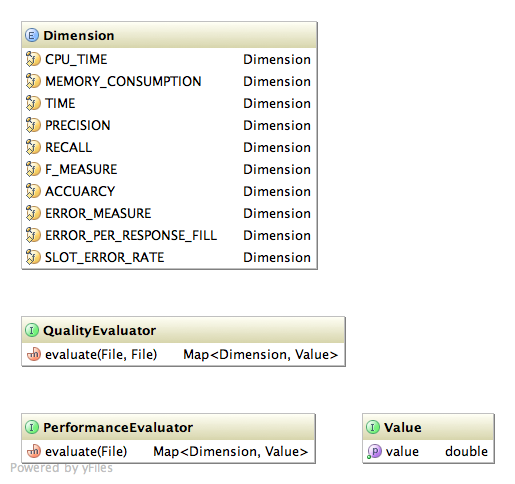
\includegraphics[width=0.8\textwidth, trim=20px 19px 0 0, clip=true]{api-evaluation.png}
\caption{Banshie Evaluation API}
\label{fig:evaluation-api}
\end{figure}

The two main service types are \texttt{QualityEvaluator} and \texttt{PerformanceEvaluator}. Both have a very similar interface, since they provide a single method to evaluate the execution result. The QualityEvaluator compares the Corpus' reference and the Extractor's hypothesis and calculates quality performance measures like Precision, Recall and F-Measure. The PerformanceEvaluator on the other hand focuses on calculating runtime performance measures, like CPU time, memory consumption and execution time by processing the event log file.

\paragraph{API Usage}
Listing \ref{lst:usage} shows the simple basic steps required to perform a single extractor execution and evaluation.

\begin{listing}[H]
\begin{minted}{java}
// via dependency injection or direct instantiation
final ExtractorRepository extractors = ...;
final CorpusRepository corpora = ...;
final Engine engine = ...;
final PerformanceEvaluator performance = ...;
final QualityEvaluator quality = ...;

final Extractor extractor = extractors.get(extractorId);
final Corpus corpus = corpora.get(corpusId);

final ExecutionResult result = engine.execute(extractor, corpus);
final Map<Dimension, Value> p = 
    performance.evaluate(result.getLogFile());
final Map<Dimension, Value> q = 
    quality.evaluate(corpus.getReference(), result.getOutput());

// handle evaluation results
...
\end{minted}
\caption{Banshie API usage}
\label{lst:usage}
\end{listing}

\subsection{Extractor interface specification}
\label{sec:extractor-specification}
Since Banshie aims to evaluate the extraction quality as well as the runtime performance of information extraction systems, it sets some special requirements for extractors.

Any extractor evaluated by the framework is required to be written in Java and compiled as a single executable Jar file for Java 1.6 or higher. Being packaged as a single file requires the extractor to bundle every external dependency into a single archive. Embedding third-party java libraries can be accomplished by utilizing the \textit{JarJar}\footnote{\url{https://code.google.com/p/jarjar/}} tool. External files, like models and training data, can be packaged as standard classpath resources.

For a Jar file to be executable it has to have a manifest file, i.e. META-INF/MANIFEST.MF), and a manifest header as shown in the following listing:

\begin{listing}[H]
\texttt{Main-Class: org.whiskeysierra.banshie.example.opennlp.Main}
\caption{Extractor manifest header}
\end{listing}

The extractor can then be started using the following command: \\ \texttt{java -jar extractor.jar}

Since an extractor under evaluation has a single input, the test document, and a single output, the annotated hypothesis, the natural choice was to utilize standard streams, standard input (\textit{stdin}) and standard output (\textit{stdout}) respectively. The test document is passed to the extractor as plain text in UTF-8 encoding. Whether the extractor streams the document or reads it into memory as a whole is up to the extractor. The output format is \gls{XML} as defined by the schema shown in listing \ref{lst:xml-schema}.

It should be explicitly stated, that this approach, in its current, form only supports single document extraction.

\begin{listing}[H]
\inputminted{xml}{../../../../../banshie-api/src/main/resources/schema.xsd}
\caption{Banshie XML Schema}
\label{lst:xml-schema}
\end{listing}

As shown in listing \ref{lst:xml-example}, the defined output format is a very simple XML document containing the original document and all found entities annotated with the corresponding type as a simple XML element tag.

\begin{listing}[H]
\inputminted{xml}{../../../../../banshie-api/src/main/resources/example.xml}
\caption{Banshie XML Example}
\label{lst:xml-example}
\end{listing}

The span element has three attributes: \texttt{type}, \texttt{start} and \texttt{end}. Type is one of \texttt{person}, \texttt{organization}, \texttt{date} or \texttt{location}, based on the ENAMEX tags developed for the Message Understanding Conference \cite{Grishman:1996}.

The attributes \texttt{start} and \texttt{end} define the UTF-8 character offset of the span in the original document to support character based association of spans in the reference and the predication.

\subsection{Reference-hypothesis association}
\label{sec:association}
\citeauthor{Douthat:1998} proposed the original version of the \enquote{General Greedy Mapping Algorithm} in 1998 \cite{Douthat:1998}. It's based on finding matching pairs of spans in the reference and the predication. Evaliex extended this algorithm by basing the matching on string or word similarity algorithms like Levenshtein-distance or the Jaccard-coeffecient \cite{Linsmayr:2010}. But since Banshie, in its current version, focuses solely on Named Entity Recognition, a simpler algorithm to associate reference and hypothesis has been used. Pairs are matched based on character offsets calculated from the original document. This way an extractor is required to find exact or partial matches of spans defined in the reference to score in the evaluation metrics.

\subsection{Implementation}
\label{sec:implementation}

\subsubsection{Engine}
The \textit{Engine} interface offers a single facade to executing an \texttt{Extractor} against a supplied \texttt{Corpus}. It's the Engine's responsibility to provide an independent and isolated execution environment for extractors, to manage process creation and lifecycle and collect and persist runtime events.

After an initial design draft, it was clear, that the Engine implementation will be too big for a single module. So the engine implementation was split up into multiple smaller, more maintainable modules using the module development patterns, defined by \citeauthor{Knoernschild:2012}\cite{Knoernschild:2012} and discussed in chapter \ref{sec:modularity}. The engine's submodules are described in the following chapters.

\begin{figure}[H]
\centering
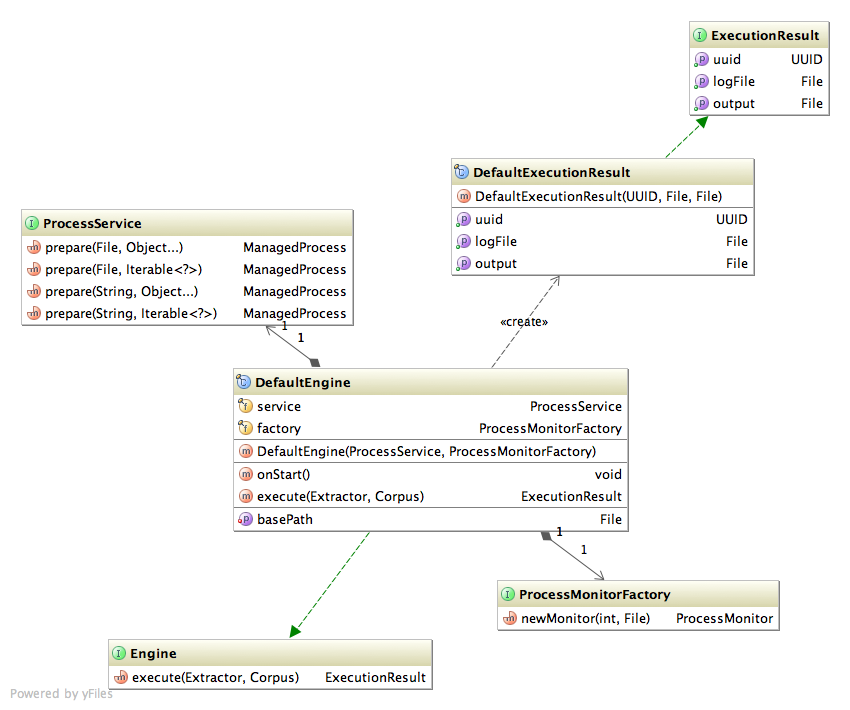
\includegraphics[width=\textwidth, trim=20px 20px 0 0, clip=true]{execution.png}
\caption{Engine implementation}
\end{figure}

\newpage
\paragraph{Process management}
The Java Process API is part of the Java Runtime Environment since version 1.0 but it has several  pitfalls, which may lead to deadlocks or zombie processes \cite{Cartmell:2009}. There even has been filed a \gls{JEP} to improve the API for controlling and managing operating system processes. \cite{JEP:102}.

Since executing an extractor in an isolated, independent execution environment is a crucial part of the Engine's task the framework required a cleaner, more fail-safe API for process creation and lifecycle management that integrates nicely with the rest of the framework and it's main general purpose library, i.e. Guava. Listing \ref{lst:process} demonstrates the minimal steps to use the  framework's Process API while figure \ref{fig:process} shows the relevant parts of it.

\begin{listing}[H]
\begin{minted}{java}
final ManagedProcess managed = service.prepare("java", "-version");
final RunningProcess process = managed.call();

// write to process.getOutput() or
// read from process.getInput()

process.await();
// or process.cancel()
\end{minted}
\caption{ProcessService API example usage}
\label{lst:process}
\end{listing}

\begin{figure}[H]
\centering
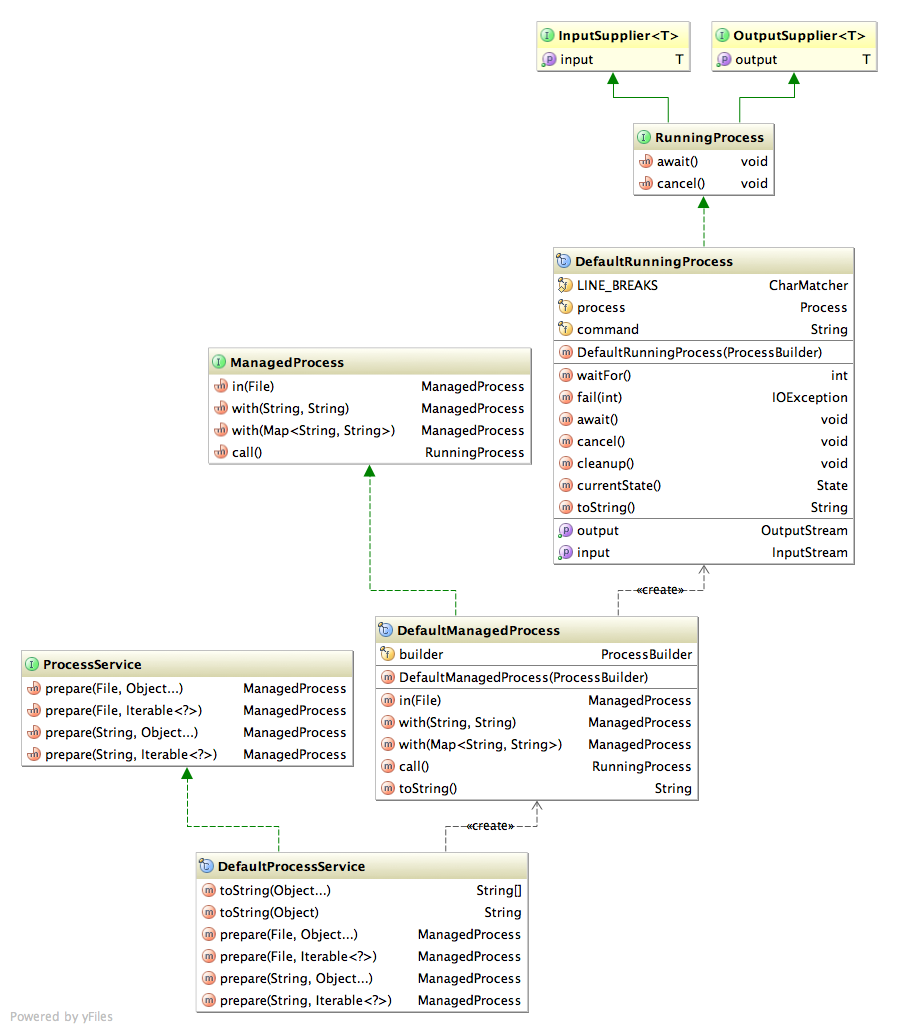
\includegraphics[width=\textwidth, trim=20px 20px 0 0, clip=true]{process.png}
\caption{ProcessService implementation}
\label{fig:process}
\end{figure}

\newpage
\paragraph{Process monitoring}
After an extractor has been started in its own environment using the ProcessService API, the operating system process needs to be monitored to ensure correct execution and to collect events, like current CPU time and memory consumption, in a periodical way, e.g. every x milliseconds.

\begin{figure}[H]
\centering
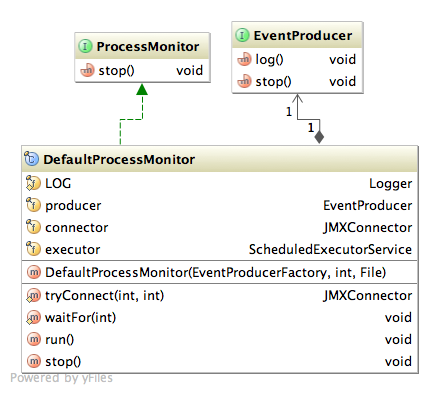
\includegraphics[width=0.8\textwidth, trim=20px 20px 0 0, clip=true]{monitor.png}
\caption{ProcessMonitor implementation}
\end{figure}

The repeated polling is realized with the JDK's built-in \\ \texttt{ScheduledExecutorService}\footnote{\url{http://docs.oracle.com/javase/6/docs/api/java/util/concurrent/ScheduledExecutorService.html}}, which schedules a special \texttt{Runnable} to run in a scheduled fashion, like shown in listing \ref{lst:scheduling}

\begin{listing}[H]
\begin{minted}{java}
executor.scheduleAtFixedRate(runnable, 0L, 1L, TimeUnit.SECONDS);
\end{minted}
\caption{Scheduling in java}
\label{lst:scheduling}
\end{listing}

\newpage
Collecting events on a separate process can be realized by using \gls{JMX}, which allows managing and monitoring java applications through a well specified and extensible interface. To allow a \gls{JMX} connection, a java process needs to be started with a special set of command line parameters as shown in listing \ref{lst:process-configuring}.

\begin{listing}[H]
\begin{minted}{java}
final ManagedProcess managed = service.prepare(
    "java",
    "-Dcom.sun.management.jmxremote",
    "-Dcom.sun.management.jmxremote.port=" + port,
    "-Dcom.sun.management.jmxremote.authenticate=false",
    "-Dcom.sun.management.jmxremote.ssl=false",
    "-jar", extractor.getPath()
);
\end{minted}
\caption{Configuring process to use JMX}
\label{lst:process-configuring}
\end{listing}

After the process has been started, a \gls{JMX} connection can be established with the following steps:

\begin{listing}[H]
\begin{minted}{java}
final String url = "service:jmx:rmi:///jndi/rmi://localhost:" + 
    port + "/jmxrmi";
final JMXServiceURL serviceUrl = new JMXServiceURL(url);
final JMXConnector connector = 
    JMXConnectorFactory.connect(serviceUrl, null);
\end{minted}
\caption{JMX connection}
\label{lst:jmx}
\end{listing}

The default implementation of the \texttt{ProcessMonitor} interface delegates the work of creating events to another service, the \texttt{EventProducer}, by passing on the \texttt{JMXConnector}.

It's worth mentioning that relying on \gls{JMX} for measuring performance values of an external extraction process is the reason why Banshie is currently limited to JVM-based extractors.

\newpage
\paragraph{Event production}
\begin{figure}[H]
\centering
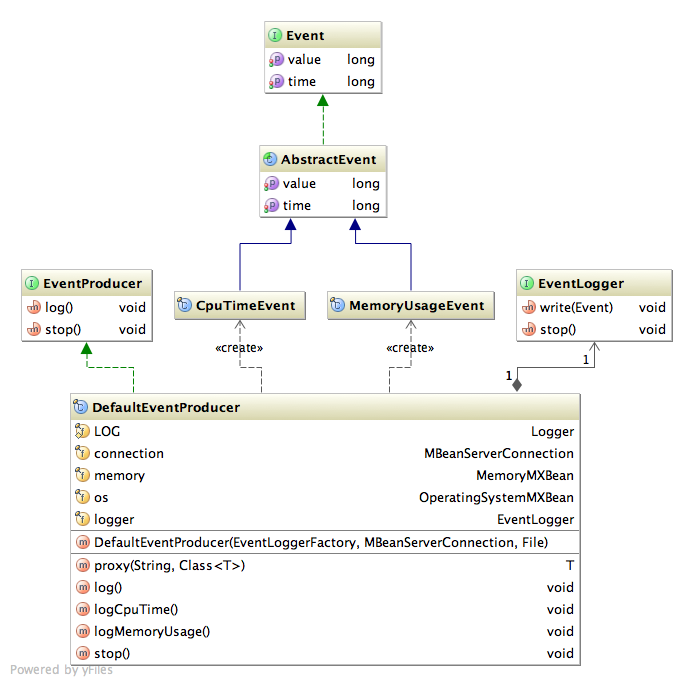
\includegraphics[width=0.95\textwidth, trim=20px 20px 0 0, clip=true]{event.png}
\caption{EventProducer implementation}
\end{figure}

It's the \texttt{EventProducer}'s responsibility to retrieve runtime performance figures by calling the corresponding \gls{JMX} endpoints and to create and populate the suitable \texttt{Event} instances. The producer generates \gls{JMX} proxies for the \texttt{MemoryMXBean}\footnote{\url{http://docs.oracle.com/javase/6/docs/api/java/lang/management/MemoryMXBean.html}} and \texttt{OperatingSystemMXBean}\footnote{\url{http://docs.oracle.com/javase/6/docs/jre/api/management/extension/com/sun/management/OperatingSystemMXBean.html}} classes, creates \texttt{CpuTimeEvent}s and \texttt{MemoryUsageEvent}s and delegates their persistence to the \texttt{EventLogger} service.

\paragraph{Event persistence}
Once events have been created, they need to be persisted on the file system to allow processing them during evaluation later on. Event persistence in Banshie is provided by the default \texttt{EventLogger} implementation, which creates a single text-oriented log file using the \gls{JSON} data format. \texttt{Event}s are serialized using \gls{JSON} mapping capabilities of the Jackson\footnote{\url{http://jackson.codehaus.org/}} library. The resulting event log file contains one \gls{JSON} entity per line.

Using \gls{JPA} for persisting events would have certainly been an option, but using a text-based logfile approach has its advantages. First of all, it's more resource friendly to stream text to a file than it is to go through several layers of abstraction to access a database via \gls{JPA}. Another reason to use \gls{JSON} for serializing is the flexibility it provides; one could easily add more information to events in the future by just extending the \gls{JSON} structure with additional key-value pairs.

\begin{figure}[H]
\centering
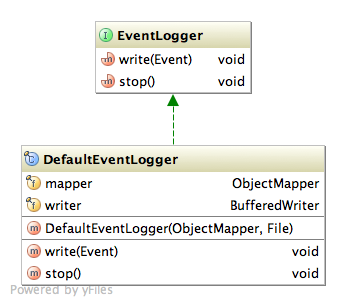
\includegraphics[width=0.65\textwidth, trim=20px 19px 0 0, clip=true]{logging.png}
\caption{EventLogger implementation}
\end{figure}

\begin{listing}[H]
\begin{minted}{javascript}
{"type":"cpu","time":1362932786442,"value":630000000}
{"type":"memory","time":1362932786870,"value":21402296}
{"type":"cpu","time":1362932787374,"value":1160000000}
{"type":"memory","time":1362932787399,"value":34213984}
{"type":"cpu","time":1362932788375,"value":2620000000}
{"type":"memory","time":1362932788423,"value":90823392}
{"type":"cpu","time":1362932789375,"value":3790000000}
{"type":"memory","time":1362932789383,"value":162860136}
{"type":"cpu","time":1362932790375,"value":6810000000}
{"type":"memory","time":1362932791603,"value":239290480}
{"type":"cpu","time":1362932791612,"value":6880000000}
{"type":"memory","time":1362932791614,"value":240990136}
{"type":"cpu","time":1362932792374,"value":7840000000}
{"type":"memory","time":1362932792376,"value":304883808}
{"type":"cpu","time":1362932793375,"value":9110000000}
{"type":"memory","time":1362932793378,"value":313170504}
\end{minted}
\caption{Example event log file excerpt}
\label{lst:event-log}
\end{listing}

\newpage
\subsubsection{Quality evaluation}
The default \texttt{QualityEvaluator} implementation has serveral tasks. It needs to map the prediction to the reference, count true positives, false positives, false negatives, run configured scoring metrics and collect their results.

\begin{figure}[H]
\centering
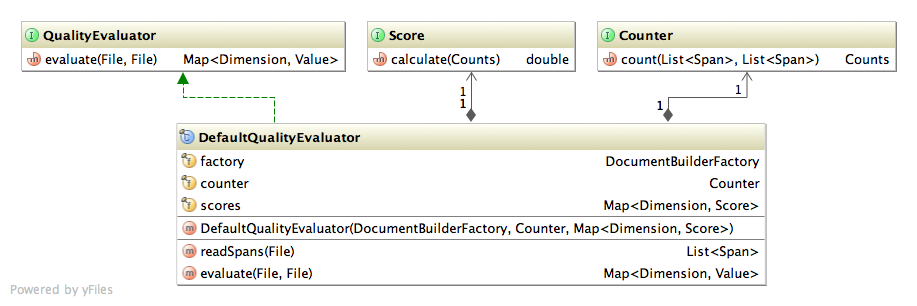
\includegraphics[width=\textwidth, trim=20px 20px 0 0, clip=true]{quality-evaluation.png}
\caption{QualityEvaluator implementation}
\end{figure}

The reference-hypothesis association is provided by the \texttt{Counter} class, as shown in figure \ref{fig:counter}. For details about the reference-hypothesis association algorithm used, please consult chapter \ref{sec:association}.

\begin{figure}[H]
\centering
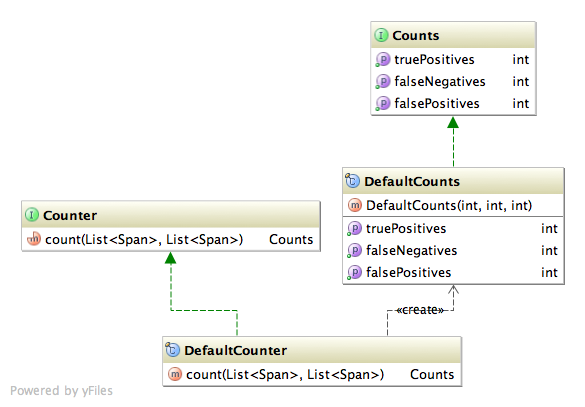
\includegraphics[width=0.8\textwidth, trim=20px 20px 0 0, clip=true]{counter.png}
\caption{Counter implementation}
\label{fig:counter}
\end{figure}

The scoring metrics are realized by implementations of the \texttt{Score} interface. Every performance metric discussed in chapter \ref{sec:evaluation-methodology} has been implemented as single \texttt{Score} implementation.

\begin{table}[H]
\centering
\begin{tabular*}{\textwidth}{ll}
	\toprule
	Metric & Implementation class \\
	\midrule
	Precision ($\rho$) & \texttt{Precision} \\
	Recall ($\pi$) &  \texttt{Recall} \\
	F-measure (\textit{F}) & \texttt{FMeasure} \\
	Error measure (\textit{E}) & \texttt{ErrorMeasure} \\
	Error per response fill (\textit{ERR}) & \texttt{ErrorPerResponseFill} \\
	Slot error rate (\textit{SER}) & \texttt{SlotErrorRate} \\
	\bottomrule
\end{tabular*}
\caption{Metric implementations}
\end{table}

Since several metrics are based on others, implementations are free to reuse instances of other types as shown in the following package diagram.

\begin{figure}[H]
\centering
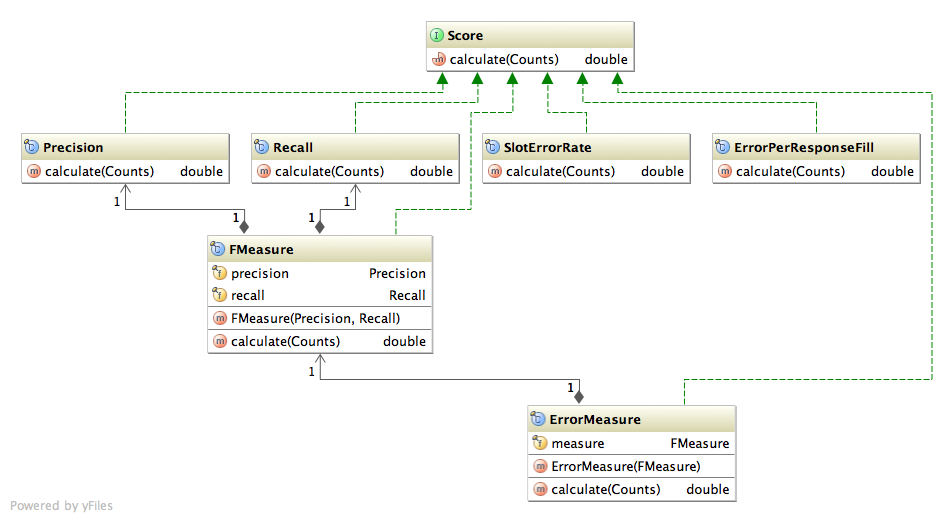
\includegraphics[width=\textwidth, trim=20px 20px 0 0, clip=true]{score.png}
\caption{Score implementation}
\end{figure}

Listing \ref{lst:recall} shows an example \texttt{Score} implementation, in this case \texttt{Recall}.

\begin{listing}[H]
\begin{minted}{java}
final class Recall implements Score {

    @Override
    public double calculate(Counts counts) {
        final double sum = counts.getTruePositives() + 
            counts.getFalseNegatives();

        if (sum > 0) {
            return counts.getTruePositives() / sum;
        } else {
            // cannot divide by zero, return error code
            return Double.NaN;
        }
    }

}
\end{minted}
\caption{Recall score implementation}
\label{lst:recall}
\end{listing}

\newpage
\subsubsection{Performance evaluation}
\begin{figure}[H]
\centering
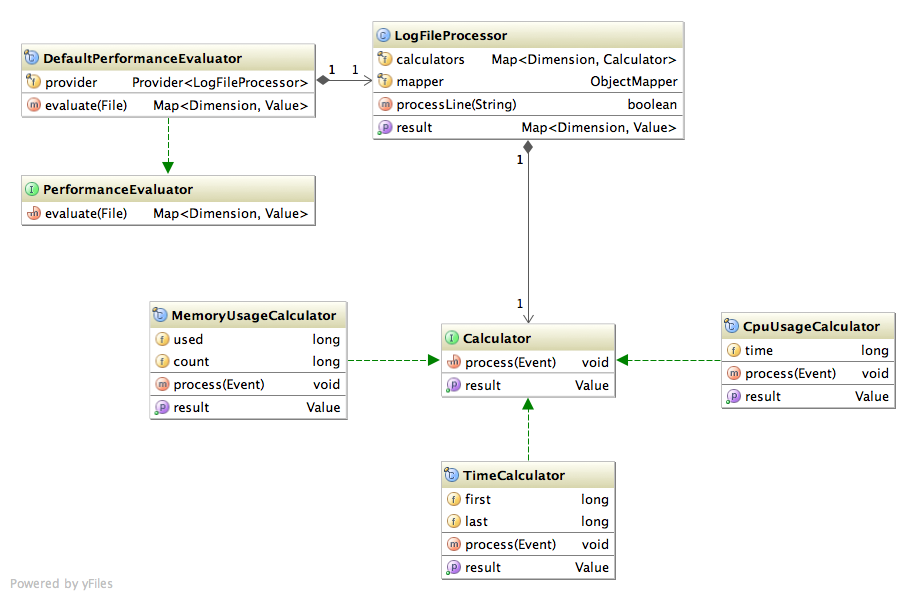
\includegraphics[width=\textwidth, trim=20px 20px 0 0, clip=true]{performance-evaluation.png}
\caption{PerformanceEvaluator implementation}
\end{figure}

Runtime performance evaluation is a little bit easier than quality evaluation. The default \texttt{PerformanceEvaluator} implementation needs to read the event log file line by line, deserialize events, update all configured calculators and finally collect their results.

\begin{listing}[H]
\begin{minted}{java}
@Override
public boolean processLine(String line) throws IOException {
    final Event event = mapper.readValue(line, Event.class);

    for (Calculator calculator : calculators.values()) {
        calculator.process(event);
    }

    return true;
}
\end{minted}
\caption{LogFileProcessor}
\end{listing}

A \texttt{Calculator} is similar to the \texttt{Score} interface shown earlier, except that calculators are inherently stateful.

\begin{listing}[H]
\begin{minted}{java}
interface Calculator {

    void process(Event event);

    Value getResult();

}
\end{minted}
\caption{Calculator Interface}
\label{lst:calculator}
\end{listing}

Banshie, in its current version, ships with three different \texttt{Calculators}:

\begin{itemize}
	\item \textbf{\texttt{CpuUsageCalculator}} \\
		Retrieves the CPU time from a stream of events.
	\item \textbf{\texttt{MemoryUsageCalculator}} \\
		Calculates the average memory consumption in megabytes.
	\item \textbf{\texttt{TimeCalculator}} \\
		Calculates the total execution time in milliseconds.
\end{itemize}

\newpage
Listing \ref{lst:memory-calculator} demonstrates a common \texttt{Calculator} implementation at the example of the \texttt{MemoryUsageCalculator} which computes the average memory consumption in megabytes.

\begin{listing}[H]
\begin{minted}{java}
final class MemoryUsageCalculator implements Calculator {

    private long used;
    private long count;

    @Override
    public void process(Event e) {
        if (e instanceof MemoryUsageEvent) {
            final MemoryUsageEvent event = 
                MemoryUsageEvent.class.cast(e);

            used += event.getValue() / 1024L / 1024L;
            count++;
        }
    }

    @Override
    public Value getResult() {
        return new SimpleValue(used / count);
    }

}
\end{minted}
\caption{MemoryUsageCalculator}
\label{lst:memory-calculator}
\end{listing}

\subsection{Summary}
This chapter described the development of Banshie, an extensible and modular evaluation framework for information extraction systems and also showed how the findings from chapter \ref{sec:evaluation-methodology} (\nameref{sec:evaluation-methodology}) and \ref{sec:modularity} (\nameref{sec:modularity}) influenced the overall system design and fundamental architecture of the framework. Various design and implementation details have been discussed, such as the API, the extractor interface specification, the output format definition as well as the reference-hypothesis association algorithm and all relevant modules, including their respective requirements and interfaces.

